\documentclass{article}

\usepackage{tikz}

% tikz packages
\usetikzlibrary{
  positioning,
  shapes.misc,
  calc,
  graphs,
  arrows.meta,
}

\tikzset{
  node distance= 5mm and 5mm,
  text height=1.5ex,
  text depth=.25ex,
  >={Stealth[round]},
  every new ->/.style={
    shorten >=1pt,
    thick, 
    black!50, 
    text=black
  },
  graphs/every graph/.style={edges=rounded corners},
  node/.style={
    rectangle,
    minimum size=6mm,
    very thick,
  },
  nonterminal/.style={
    node,
    draw=red!50!black!50,
    top color=white,
    bottom color=red!50!black!20,
    font=\itshape,
  },
  terminal/.style={
    node,
    rounded corners=3mm,
    draw=black!50,
    top color=white,
    bottom color=black!20,
    font=\ttfamily,
  },
}

\begin{document}
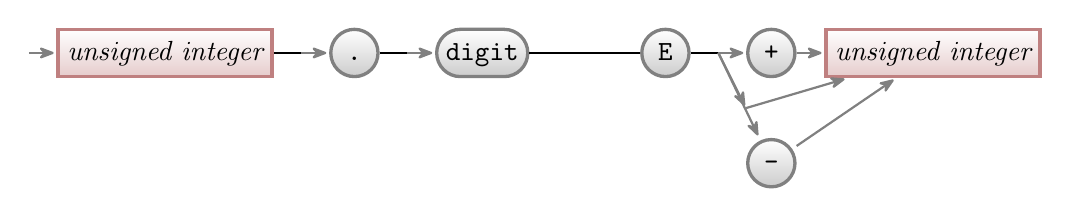
\begin{tikzpicture}
  \graph [grow right sep, branch down=7mm] {
    /                 [coordinate]  ->
    unsigned integer  [nonterminal] --
    p1                [coordinate]  ->
    "."               [terminal]    -- 
    p2                [coordinate]  ->
    digit             [terminal]    --
    p3                [coordinate]  --
    p4                [coordinate]  --
    p5                [coordinate]  --
    E                 [terminal]    -- 
    q1                [coordinate]  ->
    {
      "+" [terminal],
      ""  [coordinate],
      "-" [terminal]
    } ->
    /unsigned integer[nonterminal]
  };
\end{tikzpicture}
\end{document}